\clearpage

\subsection{Conclusions}
\begin{tcolorbox}	
\begin{tabular}{p{2.75cm} p{0.2cm} p{10.5cm}} 	
\textbf{Student Name}  &:& Tiago Esteves    (October 03, 2017 - )\\
\textbf{Goal}          &:& Conclusions about the ILPs created and their results.
\end{tabular}
\end{tcolorbox}
\vspace{11pt}

After realizing the ILP models for the three transport modes we will focus on these results obtained and draw as many conclusions as possible from these results. For this, the figure \ref{graphic_comparative} is created with the information obtained previously.

\begin{figure}[h!]
\centering
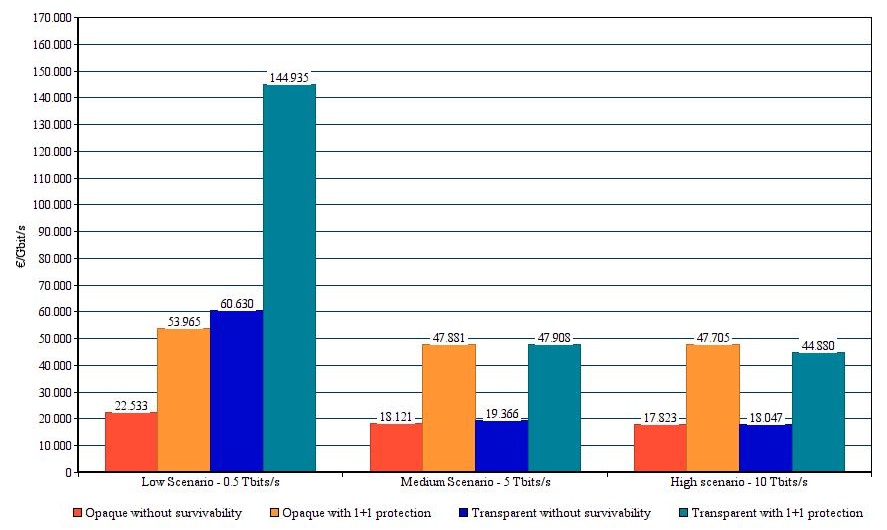
\includegraphics[width=\textwidth]{sdf/ilp/figures/comparative_image}
\caption{Graphic with the cost in Euros per Gbit/s of the three modes of transport without survivability and with 1+1 protection for all scenarios referred initially.}
\label{graphic_comparative}
\end{figure}

Through the previous figure we can draw several conclusions such as:
Regardless of the transport mode and the type of survivability, it is clear that the higher the network traffic, the lower the cost per Gbit/s.
The cost with 1+1 protection is always more than twice the cost without protection regardless of the mode of transport used.
%It is possible to state that the translucent transport mode has a cheaper cost compared to the other two modes of transport, regardless of network traffic and type of survival.
Regarding the low scenario it is possible to state that the transparent mode has a much higher cost than other modes of transport.
In relation to the other two scenarios it is possible to state that the opaque and transparent mode have a similar cost regardless of the mode of survivability. In the last scenario transparent mode with protection has a cost per bit lower than opaque transport mode.
